% put all Mike's macros in and begin document
\documentclass[pdftex]{article}
\usepackage[pdftex]{graphics}
\usepackage{subfigure}
\usepackage{hhline}
\usepackage[usenames,dvipsnames]{color}
\usepackage{colortbl}
\usepackage[screen,pdftex]{mcdlecture}
\newcommand{\bs}{\relax}
\newcommand{\es}{\newpage}
\fboxsep=.01\textwidth \fboxrule=1pt
\newsavebox{\savepar}
\newenvironment{boxit}{\begin{lrbox}{\savepar}
    \begin{minipage}[b]{0.975\textwidth}}
    {\end{minipage}\end{lrbox}\framebox{\usebox{\savepar}}}


%%%%%%%%%%%%%%%%%%%%%%%%%%%%%%%%%%%%%%%%%%%%%%%%%%%%%%%%%%
%% THE FOLLOWING ARE THINGS THAT WE MIGHT CHANGE FROM YEAR TO YEAR OR
%% VENUE TO VENUE
    \lhead{MCMC in Statistical Genetics}
    \lfoot{Dr Eric C. Anderson and Dr Matthew Stephens}
%	\lfoot{Dr Eric C. Anderson and Dr John Novembre}
%    \rfoot{UW - Summer Institute, July 2013}
%	 \rfoot{Edinburgh - European Institute, June 2012}
\rfoot{Brazil - Summer Institute, February 2014}

% on this one, be sure to update the venue and the module number
%\newcommand{\coursetitlepage}{European Institute in Statistical Genetics
%\newcommand{\coursetitlepage}{Summer Institute in Statistical Genetics
\newcommand{\coursetitlepage}{Brazilian Edition of the Summer \\Institute in Statistical Genetics

Module 9:

MCMC for Genetics}

%% Then update the schedule.  Note that I have broken that
%% out into a separate file like: schedule_table_edinburgh2012.tex
%% which is input in Overview.tex

%% Then be sure to change any time-sensitive events in the 
%% probability discussion in Matthew's first lecture.

%% And also update "structure_fun" link to my wiki to the right
%% year and venue.
%%%%%%%%%%%%%%%%%%%%%%%%%%%%%%%%%%%%%%%%%%%%%%%%%%%%%%%%%%


\begin{document}

\DeclareGraphicsExtensions{.jpg,.pdf,.png}%



%% Eric added a few things:
% some commands that Eric made for making a title while starting
% a new lecture and for making titles of new slides.
\newcommand{\newlecture}[1]{\newpage\begin{center}\section*{#1}\end{center}}
\newcommand{\newslide}[1]{\newpage\subsection*{#1: \hfil}}
 \newcommand{\Exp}{\Bbb{E}}
 \newcommand{\Var}{{\mathrm{Var}}}
 %% Some pretty etc.'s, etc...
\newcommand{\cf}{{\em cf.}}
\newcommand{\eg}{{\em e.g.},}
\newcommand{\ie}{{\em i.e.},}
\newcommand{\etal}{{\em et al.}\ }
\newcommand{\etc}{{\em etc.}}

%% some handy things for making bold math
\def\bm#1{\mathpalette\bmstyle{#1}}
\def\bmstyle#1#2{\mbox{\boldmath$#1#2$}}
\newcommand{\thh}{^\mathrm{th}}
\newcommand{\bpi}{{\pi}}
\newcommand{\mP}{\mathbf{P}}




\rhead{Session 4 - \thepage}




% each \include command puts a new file in.

% to make typesetting faster while working on a single
% section, but still have the appropriate page numbering
% and references, use the \includeonly command



\newlecture{Markov Chain Monte Carlo: \\  more complex examples}
Goals of this lecture:
\begin{itemize}
\item Consider MCMC in more than a single dimension
\item Describe component-wise Metropolis-Hastings sampling 
\item Introduce the idea of latent variables and show how they lend themselves to Gibbs sampling---a special case of component-wise M-H sampling
\end{itemize}

\newslide{Genotype Frequencies and Inbreeding}
Starting with the last exercise of Session~3: one locus with two alleles, $A$ and $a$, at frequencies $p$ and $1-p$, respectively, and ``inbreeding coefficient'' $f$.

Probabilities of the three genotypes are:
\begin{itemize}
\item $P(AA) = fp + (1-f)p^2$
\item $P(Aa~\mathrm{or}~aA) = (1-f)2p(1-p)$
\item $P(aa) = f(1-p) + (1-f)(1-p)^2$
\end{itemize}

Since ``inbreeding'' is used to describe a lot of (related) things, let's briefly review what this model is saying\ldots




%%%% INBREEDING DIAGRAMS
\newslide{Inbreeding model}
\enlargethispage*{1000pt}
\begin{minipage}[c]{.45\textwidth}
\begin{center}
Not-inbred with probability \\
$1-f$

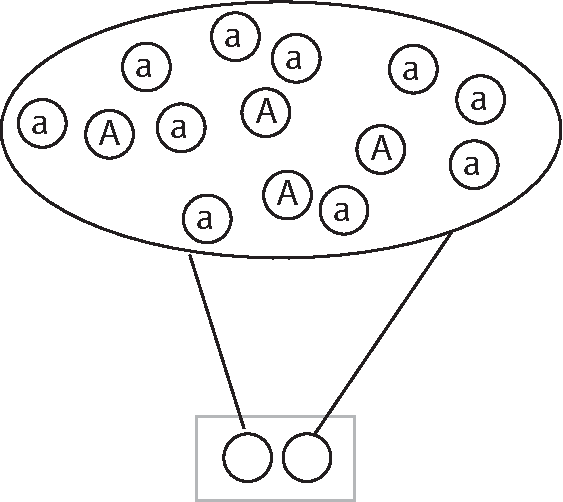
\includegraphics[width=.8\textwidth]{illus/SimpleNotInbreeding.pdf}
\end{center}
\begin{itemize}
\small
\item $P(AA) = p^2$
\item $P(Aa~\mathrm{or}~aA) = 2p(1-p)$
\item $P(aa) = (1-p)^2$
\end{itemize}

\end{minipage}
\hfill
\begin{minipage}[c]{.45\textwidth}
\begin{center}
Inbred with probability \\
$f$

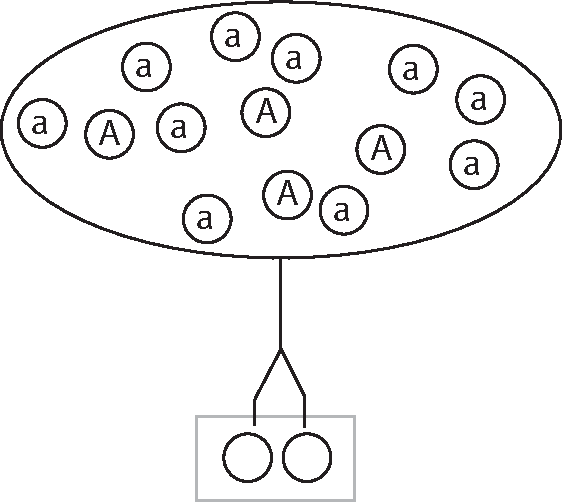
\includegraphics[width=.8\textwidth]{illus/SimpleInbreeding.pdf}
\end{center}
\begin{itemize}
\small
\item $P(AA) = p $
\item $P(Aa~\mathrm{or}~aA) = 0$
\item $P(aa) = (1-p)$
\end{itemize}
\end{minipage}
\hrule
{\small
\begin{eqnarray*}
P(n_{AA},n_{Aa},n_{aa}|p,f) &=& C\times [fp + (1-f)p^2]^{n_{AA}} \times [(1-f)2p(1-p)]^{n_{Aa}} \\
 &\times & [ f(1-p) + (1-f)(1-p)^2]^{n_{aa}}
\end{eqnarray*}
}




\newslide{What Our Data Would Look Like}
\begin{itemize}
\item We have a sample of $n$ individuals total.
\begin{itemize}
\item $n_{AA}$ are homozygous for the $A$ allele
\item $n_{Aa}$ are heterorozygous
\item $n_{aa}$ are homozygous for the $a$ allele
\end{itemize}
\item Clearly, $n=n_{AA} + n_{Aa} + n_{aa}$
\end{itemize}

A concrete example we will use throughout this lecture is $n=50$ with:
\[
n_{AA}=30~~~~~~~~~~~~~n_{Aa}=10~~~~~~~~~~~~~n_{aa}=10
\]
which are roughly the expected values if $p=.7$ and $f=.5$.




%%BAYESIAN SPECIFICATION FOR ESTIMATING f and p
\newslide{Bayesian Model for Estimating $f$ and $p$}
To go about estimating $f$ and $p$ in a Bayesian fashion, we must fully specify the model.  This means that we need 
\begin{itemize}
\item Priors for $f$ and $p$.  We will choose uniform priors $f\sim\mathrm{Beta}(1,1)$ and $p\sim\mathrm{Beta}(1,1)$
\item The data themselves.  These are $n_{AA}$, $n_{Aa}$, and $n_{aa}$.
\item The likelihood: $P(n_{AA},n_{Aa},n_{aa}|p,f)$, which is given on the previous page
\end{itemize}
The posterior distribution is then prior $\times$ likelihood, divided by the (``nasty'') normalizing constant
\[
P(p,f|n_{AA},n_{Aa},n_{aa}) = \frac{P(f)P(p)P(n_{AA},n_{Aa},n_{aa}|p,f)}{\int_{f,p}P(f)P(p)P(n_{AA},n_{Aa},n_{aa}|p,f)dfdp}
\]


\newpage
Computing the normalizing constant is difficult, but with MCMC, {\em we don't have to!}

Recall, to perform MCMC it suffices to know the target distribution up to a constant of proportionality. 

Our target distribution is 
\[
P(p,f|n_{AA},n_{Aa},n_{aa}) \propto P(f)P(p)P(n_{AA},n_{Aa},n_{aa}|p,f)
\]
So long as $0< f< 1$ and $0<p<1$.

Otherwise it is 0.


\newslide{Two-Dimensional M-H Sampler}
We can compute the target distribution (up to a constant) easily for any $f$ and $p$.   So, to simulate from this posterior distribution we can just implement a Metropolis-Hastings sampler.  

Following the examples of Session~3, for $p$ we will choose a normal proposal distribution centered on the current value with standard deviation of $s_p$:
\[
	q(p^*|p) \equiv \mathrm{Normal}(p,s_p)
\]
And, we will use the same for $f$:
\[
	q(f^*|f) \equiv \mathrm{Normal}(f,s_f)
\]

Applying these proposal distributions in sequence gives us a simple way to simulate proposed values, $(p^*,f^*)$, from the current values $(p,f)$.

\newpage

A ``sweep'' of our MCMC algorithm would look like:
\begin{enumerate}
\item Propose a new value, $(p^*,f^*)$ for $(p,f)$
\begin{itemize}
\item propose $p^*$ from $\mathrm{Normal}(p,s_p)$
\item propose $f^*$ from $\mathrm{Normal}(f,s_f)$
\end{itemize}
\item Accept or reject the proposed value $(p^*,f^*)$ with probability $R$ which is the minimum of 1 and the Hasting's Ratio:
\end{enumerate}
\[
\small
R=\min\biggr\{1,
\frac{q(p|p^*)q(f|f^*)}{q(p^*|p)q(f^*|f) } \times 
\frac{P(p^*)P(f^*)P(n_{AA},n_{Aa},n_{aa}|p^*,f^*)}{P(p)P(f)P(n_{AA},n_{Aa},n_{aa}|p,f)}
\biggl\}
\]
If you accept the proposed value, set the current value to the proposed value.  Otherwise leave the current values unchanged.

\fbox{Computer Demo}


\newslide{Component-wise Metropolis Hastings Sampler  }
\begin{itemize}
\item In any MCMC implementation, the proposal distribution {\em need not propose changes to {\bf every} variable/parameter  in the model}.
\item In fact, there are few ``real-world'' problems requiring MCMC in which you would use a single proposal distribution in which changes were proposed to all the variables in the model.
\item {\bf Important Concept:}
\begin{itemize}
\item Any proposal distribution, regardless of how many or how few variables it proposes changes to, is valid, so long as the proposal is accepted or rejected in a way that satisfies detailed balance w.r.t.\ the target distribution.
\item These different flavors of the ``propose-reject/accept'' step may be combined in series in whatever manner is desired, so long as they produce an irreducible, aperiodic chain\footnote{Nonetheless, some ways are better than others and will lead to a better-mixing chain}. 
\end{itemize}
\end{itemize}


\newslide{Simple Component-wise M-H Sampler for $p$ and $f$}
Simplest scenario has a sweep as follows:
\begin{enumerate}
\item Do an update for \textcolor{Violet}{$p$}:
\begin{enumerate}
\item propose $\textcolor{Violet}{p^*}$ from $\mathrm{Normal}(p,s_p)$
\item Accept or reject the proposed value $\textcolor{Violet}{p^*}$ with probability $\min\{1,\alpha\}$, where: 
\[
\alpha = \frac{\textcolor{Violet}{q(p|p^*)}}{\textcolor{Violet}{q(p^*|p)} } \times
\frac{\textcolor{Violet}{P(p^*)}P(f)\textcolor{Violet}{P(n_{AA},n_{Aa},n_{aa}|p^*,f)}}{\textcolor{Violet}{P(p)}P(f)\textcolor{Violet}{P(n_{AA},n_{Aa},n_{aa}|p,f)}}
\]
\end{enumerate}
\item Do an update for \textcolor{Orange}{$f$}:
\begin{enumerate}
\item propose $\textcolor{Orange}{f^*}$ from $\mathrm{Normal}(f,s_f)$
\item Accept or reject the proposed value $\textcolor{Orange}{f^*}$ with probability $\min\{1,\alpha\}$, where: 
\[
\alpha = \frac{
	\textcolor{Orange}{q(f|f^*)}}  {\textcolor{Orange}{q(f^*|f)} } \times
\frac{
	P(p)\textcolor{Orange}{P(f^*)}\textcolor{Orange}{P(n_{AA},n_{Aa},n_{aa}|p,f^*)}}
{P(p)\textcolor{Orange}{P(f)}\textcolor{Orange}{P(n_{AA},n_{Aa},n_{aa}|p,f)}}
\]
\end{enumerate}
\end{enumerate}



\newslide{Simple Component-wise M-H Sampler for $p$ and $f$, cont'd}
Some very important points:
\begin{itemize}
\item The proposals are each a little simpler (though just slightly\ldots) than jointly proposing changes to $(p,f)$
\item Neither step~1 nor step~2 of the sweep creates an irreducible chain (obviously, if you never update $p$, for example, your chain could never reach every possible value of $p$).
\item However, taken together, steps~1 and~2 create an irreducible chain.
\end{itemize}
\fbox{Computer Demo}


\newslide{Simple Component-wise M-H Sampler for $p$ and $f$, cont'd}
Two more important points
\begin{itemize}
\item The form of the Hastings ratio is a little simpler when we have proposed changing just a subset of the variables.
\item However, in this case the target density remains just as complex, because it does not factorize into a separate part for $f$ and a part for $p$.
\item Since we are changing just a small part of the model at a time, it seems like we could spend some more energy on making each separate proposal distribution more ``intelligent.''
\end{itemize}

The final two points above get us to thinking about Gibbs sampling, which we will return to after a brief discussion of latent variables\ldots






\newslide{Formulating the Model with Latent Variables}
Just think how easy it would be to estimate $f$ and $p$ if we knew whether every individual we sampled was inbred or not:
\enlargethispage*{1000pt}
\begin{center}
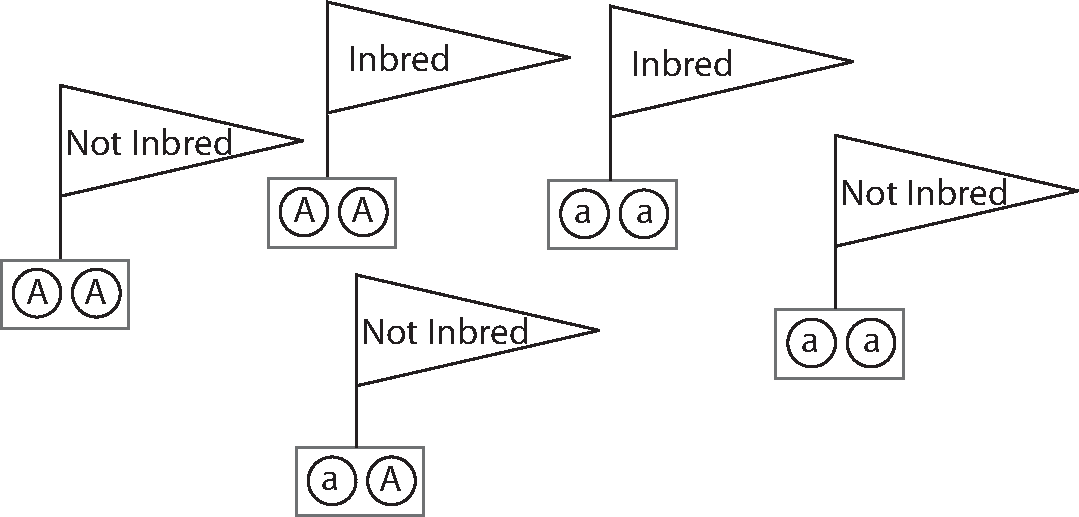
\includegraphics[width=.65\textwidth]{illus/InbreedingFlags.pdf}
\end{center}
\begin{itemize}
\item Now, $f$ is just a binomial proportion
\item To estimate $p$ you count both the alleles from Non-inbred individuals, and just one allele from Inbred individuals, and then it too is simply a binomial proportion.
\end{itemize}

\newpage

In other words, if your data look like:
\begin{center}
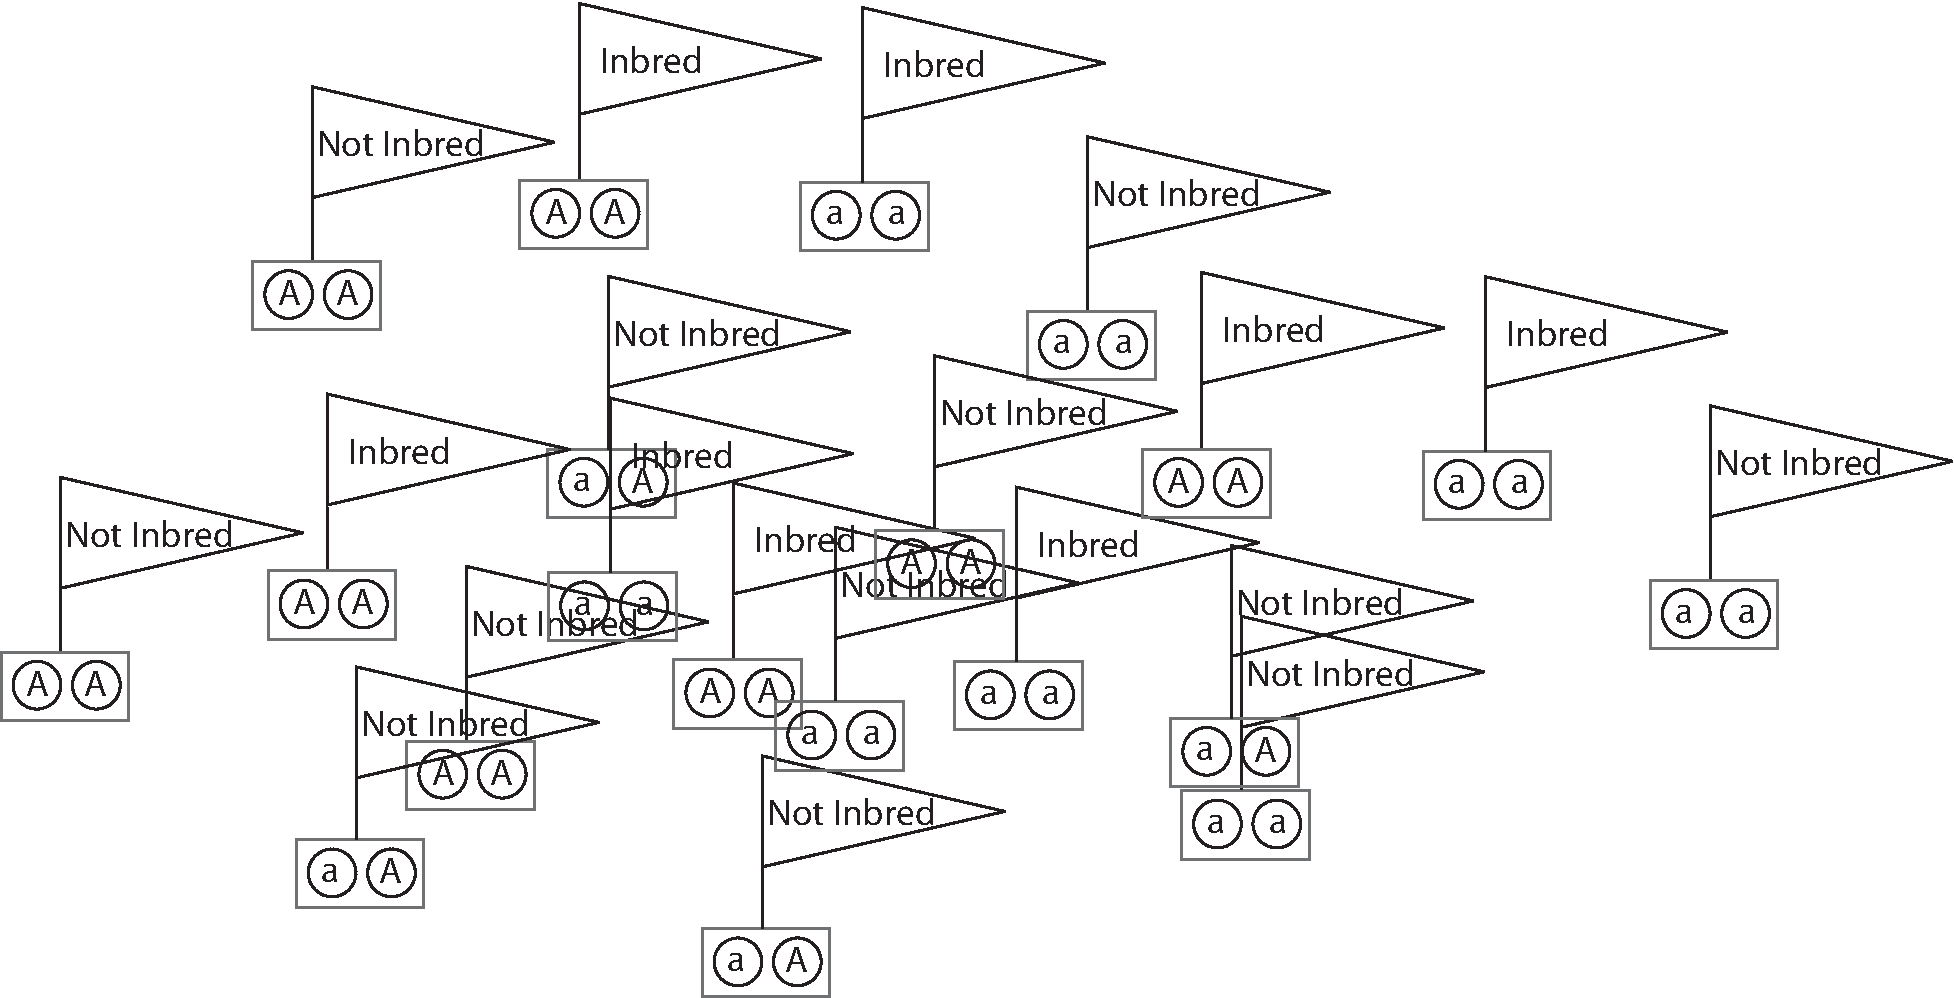
\includegraphics[width=.9\textwidth]{illus/InbreedingLotsOfFlags.pdf}
\end{center}
\ldots then, to estimate $f$, you don't even need to think about the alleles carried by anyone\ldots

\newpage
\ldots you just have to ``count the flags'':
\begin{center}
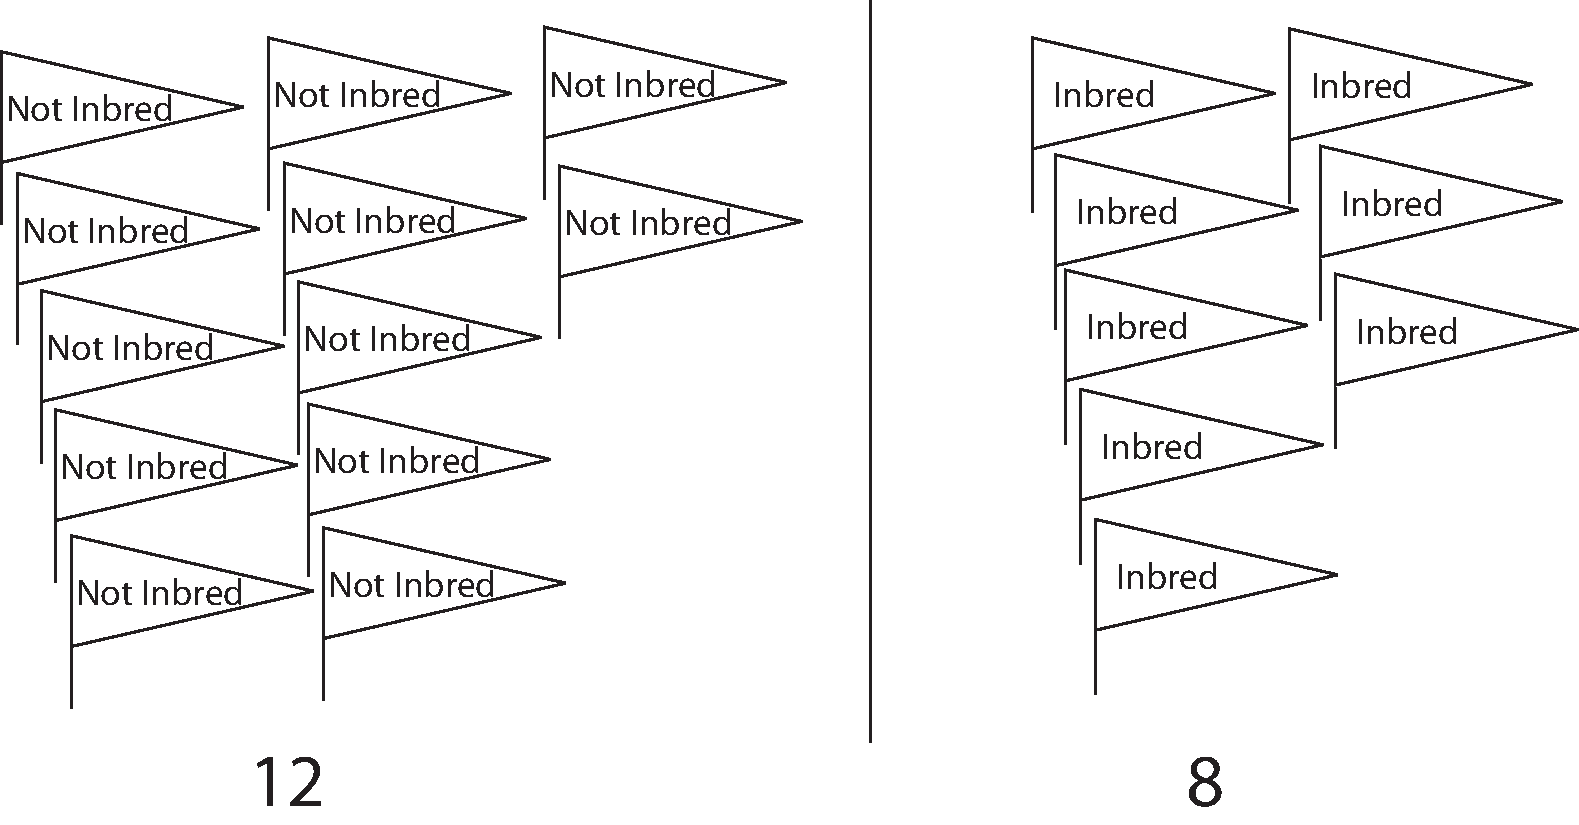
\includegraphics[width=\textwidth]{illus/InbreedingFlagsOnly.pdf}
\end{center}



\newpage
To estimate $p$ you just have to count alleles\ldots
\begin{center}
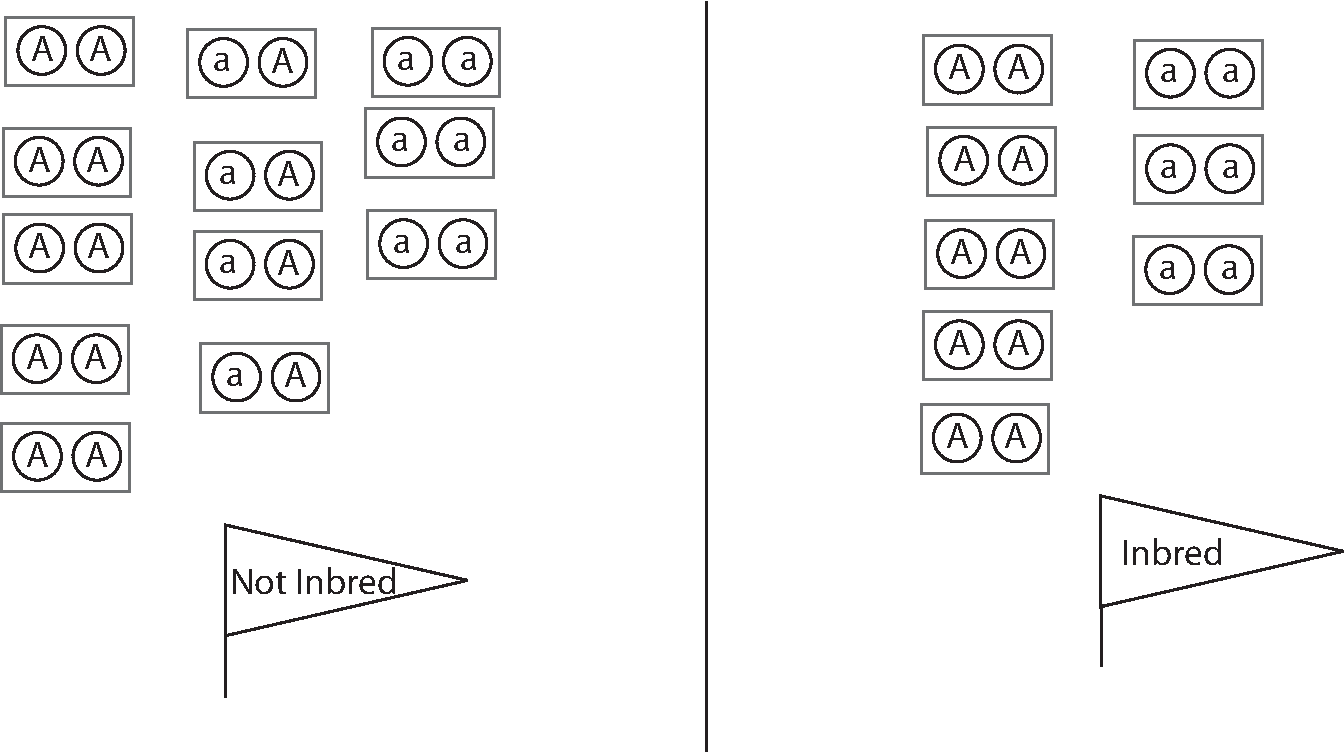
\includegraphics[width=\textwidth]{illus/InbreedingEstimating_p_1.pdf}
\end{center}

\newpage
Keeping in mind each inbred individual contributes just a single gene copy\ldots
\begin{center}
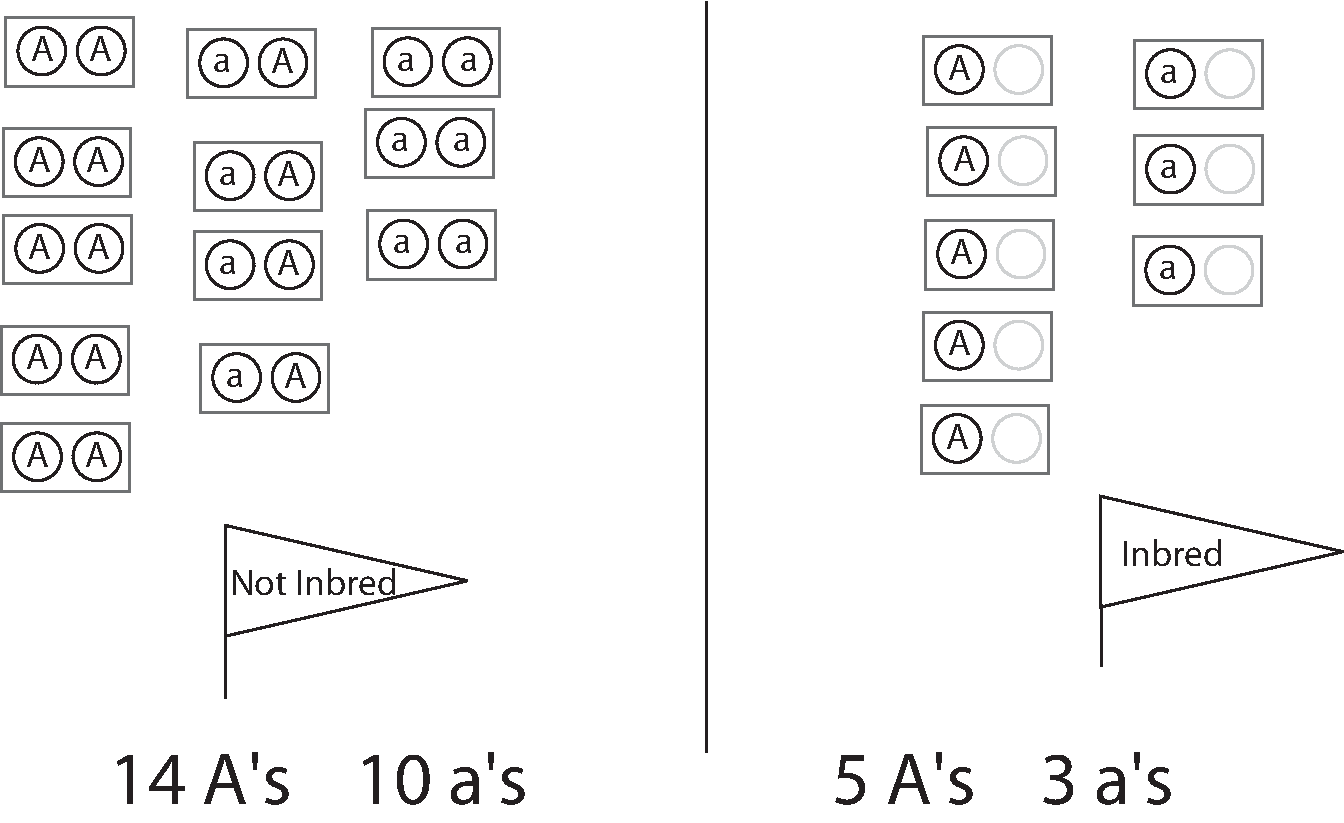
\includegraphics[width=\textwidth]{illus/InbreedingEstimating_p_2.pdf}
\end{center}



\newslide{Joint Density of $p$, $f$, and $\bm{U}$}
\begin{itemize}
\item We denote the $n$ latent variables as $\bm{U}=(U_1,\ldots,U_n)$.
\item $u_i=0$ indicates that $i$ is Not Inbred.  $u_i=1$ indicates $i$ is Inbred.
\item Let $\bm{Y}=(Y_1,\ldots,Y_n)$ denote the genotypes
\end{itemize}
So, the joint density is:
\[
P(\textcolor{Violet}{p},\textcolor{Orange}{f},\textcolor{Green}{\bm{U}},\bm{Y}) = P(\textcolor{Violet}{p})P(\textcolor{Orange}{f})P(\textcolor{Green}{\bm{U}}|\textcolor{Orange}{f}) P(\bm{Y}|\textcolor{Green}{\bm{U}},\textcolor{Violet}{p})
\]
and, so, the posterior is:
\[
P(\textcolor{Violet}{p},\textcolor{Orange}{f},\textcolor{Green}{\bm{U}}|\bm{Y}) = \frac{P(\textcolor{Violet}{p},\textcolor{Orange}{f},\textcolor{Green}{\bm{U}},\bm{Y})}
{ \int_{\textcolor{Violet}{p}} \int_{\textcolor{Orange}{f}} \sum_{0\leq  \textcolor{Green}{U_1}\leq 1}
\cdots
\sum_{0\leq  \textcolor{Green}{U_n}\leq 1}
P(\textcolor{Violet}{p},\textcolor{Orange}{f},\textcolor{Green}{\bm{U}},\bm{Y})d\textcolor{Violet}{p}d\textcolor{Orange}{f}
}
\]
The normalizing constant is even nastier!  It seems we have gained little, until we remember that we don't have to mess with the normalizing constant, \ldots but even then it's not immediately clear we have gained anything.

\newslide{Generic MCMC for $f$ and $p$ with latent variables}
\begin{itemize}
\item Recall, we wish to simulate $f$ and $p$ from their posterior distributions and so learn about $P(f,p|\bm{Y})$.
\item However, now, our chain is moving about the space of $f$, $p$, {\em and} $\bm{U}$\ldots
\begin{itemize}
\item it visits a sequence of states of the form $(f^{(1)},p^{(1)},\bm{U}^{(1)})$, $(f^{(2)},p^{(2)},\bm{U}^{(2)})$, $(f^{(3)},p^{(3)},\bm{U}^{(3)}), \ldots$
\end{itemize}
\mbox{}\vspace*{.25in}
\item {\bf Important Concept}: Obtaining the Marginal Posterior Distribution from MCMC output is simple:
\begin{itemize}
\item From the sequence $(f^{(1)},p^{(1)},\bm{U}^{(1)})$, $(f^{(2)},p^{(2)},\bm{U}^{(2)}),\ldots$ you can just focus on collecting the values $(f^{(1)},p^{(1)})$, $(f^{(2)}),\ldots$, discarding the $\bm{U}^{(\cdot)}$'s if you are not interested in their posterior distribution.  (Note, though, that you might be interested in the individual $U_i$'s!).
\end{itemize}
\end{itemize}



\newslide{Naive Metropolis-Hastings for $f$, $p$, and $\bm{U}$}
\begin{enumerate}
\item Do an update for \textcolor{Violet}{$p$}:
\begin{enumerate}
\item propose $\textcolor{Violet}{p^*}$ from $\mathrm{Normal}(p,s_p)$
\item accept or reject on the basis of 
\[
\frac{\textcolor{Violet}{q(p|p^*)}}{\textcolor{Violet}{q(p^*|p)} } \times
\frac{ P(\textcolor{Violet}{p^*})P(\textcolor{Orange}{f})P(\textcolor{Green}{\bm{U}}|\textcolor{Orange}{f}) P(\bm{Y}|\textcolor{Green}{\bm{U}},\textcolor{Violet}{p^*})}
{ P(\textcolor{Violet}{p})P(\textcolor{Orange}{f})P(\textcolor{Green}{\bm{U}}|\textcolor{Orange}{f}) P(\bm{Y}|\textcolor{Green}{\bm{U}},\textcolor{Violet}{p})}
\]
\end{enumerate}


\item Do an update for \textcolor{Orange}{$f$}:
\begin{enumerate}
\item propose $\textcolor{Orange}{f^*}$ from $\mathrm{Normal}(f,s_f)$
\item accept or reject on the basis of 
\[
\frac{\textcolor{Orange}{q(f|f^*)}}{\textcolor{Orange}{q(f^*|f)} } \times
\frac{ P(\textcolor{Violet}{p})P(\textcolor{Orange}{f^*})P(\textcolor{Green}{\bm{U}}|\textcolor{Orange}{f^*}) P(\bm{Y}|\textcolor{Green}{\bm{U}},\textcolor{Violet}{p})}
{ P(\textcolor{Violet}{p})P(\textcolor{Orange}{f})P(\textcolor{Green}{\bm{U}}|\textcolor{Orange}{f}) P(\bm{Y}|\textcolor{Green}{\bm{U}},\textcolor{Violet}{p})}
\]
\end{enumerate}
\newpage
\item Do an update for \textcolor{Green}{$\bm{U}$} ($n$ separate updates, one for each \textcolor{Green}{$U_i$}).


For $i$ in $1,\ldots,n$:
\begin{enumerate}
\item Propose a new \textcolor{Green}{$U^*_i$} by flipping a coin (heads=0, tails=1).
\item Accept or reject on the basis of 
\[
\frac{\textcolor{Green}{q(U_i|U_i^*)}}{\textcolor{Green}{q(U_i^*|U_i)} } \times
\frac{ P(\textcolor{Violet}{p})P(\textcolor{Orange}{f})P(\textcolor{Green}{\bm{U}^*}|\textcolor{Orange}{f}) P(\bm{Y}|\textcolor{Green}{\bm{U}^*},\textcolor{Violet}{p})}
{ P(\textcolor{Violet}{p})P(\textcolor{Orange}{f})P(\textcolor{Green}{\bm{U}}|\textcolor{Orange}{f}) P(\bm{Y}|\textcolor{Green}{\bm{U}},\textcolor{Violet}{p})}
\] 
\[
=
\frac{\textcolor{Green}{q(U_i|U_i^*)}}{\textcolor{Green}{q(U_i^*|U_i)} } \times
\frac{ P(\textcolor{Violet}{p})P(\textcolor{Orange}{f})P(\textcolor{Green}{U_i^*}|\textcolor{Orange}{f}) P(\bm{Y}|\textcolor{Green}{U_i^*},\textcolor{Violet}{p})}
{ P(\textcolor{Violet}{p})P(\textcolor{Orange}{f})P(\textcolor{Green}{U_i}|\textcolor{Orange}{f}) P(\bm{Y}|\textcolor{Green}{U_i},\textcolor{Violet}{p})}
\] 
\end{enumerate}
\end{enumerate}

Note the cancellations in all these Hastings Ratios.

\fbox{Computer Demo}~\footnote{which will segue into Gibbs sampling}

\newslide{Gibbs Sampling}
Gibbs sampling is a special case of the component-wise M-H sampler in which the proposal distribution is the {\em full conditional distribution}.

Gibbs Sampling Step for \textcolor{Orange}{$f$}:
\begin{itemize}
\item Recall the generic component-wise M-H update:
\[
\frac{\textcolor{Orange}{q(f|f^*)}}{\textcolor{Orange}{q(f^*|f)} } \times
\frac{ P(\textcolor{Violet}{p})P(\textcolor{Orange}{f^*})P(\textcolor{Green}{\bm{U}}|\textcolor{Orange}{f^*}) P(\bm{Y}|\textcolor{Green}{\bm{U}},\textcolor{Violet}{p})}
{ P(\textcolor{Violet}{p})P(\textcolor{Orange}{f})P(\textcolor{Green}{\bm{U}}|\textcolor{Orange}{f}) P(\bm{Y}|\textcolor{Green}{\bm{U}},\textcolor{Violet}{p})}
\]


The full conditional distribution for \textcolor{Orange}{$f$} is the distribution of \textcolor{Orange}{$f$} conditional upon the current values of all other variables in the model.  This must be proportional to the product of all the factors in the joint density that have \textcolor{Orange}{$f$} in them: $P(\textcolor{Orange}{f})P(\textcolor{Green}{\bm{U}}|\textcolor{Orange}{f})$

\newpage 
\item\begin{minipage}{.4\textwidth}
The $P(\textcolor{Green}{\bm{U}}|\textcolor{Orange}{f})$ portion of the joint density pertains to ``counting up our flags''
\end{minipage}
~~~~
\begin{minipage}{.5\textwidth}
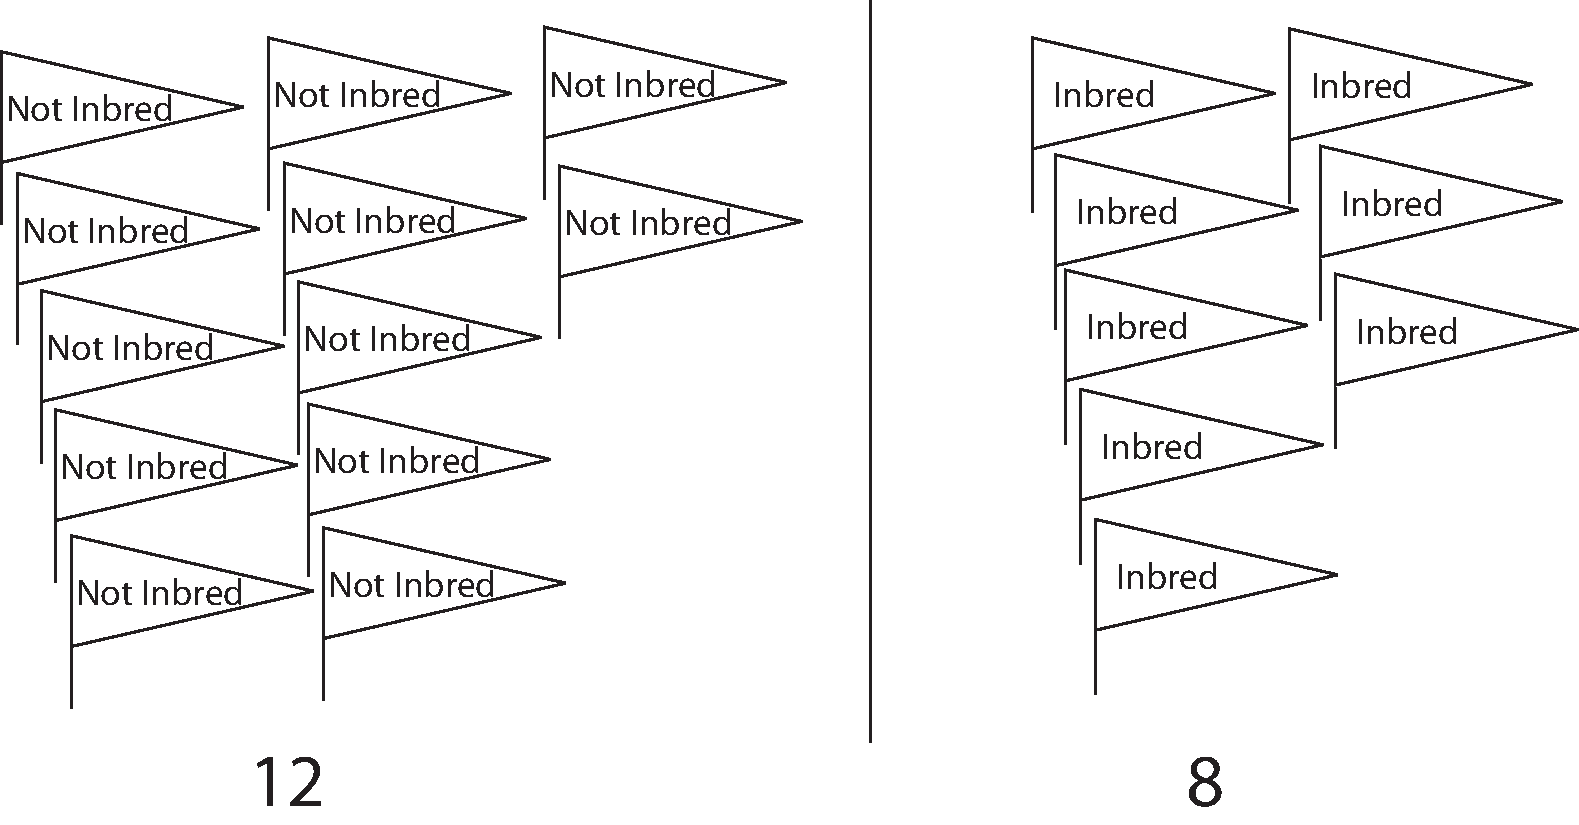
\includegraphics[width=.84\textwidth]{illus/InbreedingFlagsOnly.pdf}
\end{minipage}

\item $P(\textcolor{Orange}{f})$ is the prior for $\textcolor{Orange}{f}$

\item So the full conditional for $\textcolor{Orange}{f}$ is a beta distribution---it's the ``posterior'' for $\textcolor{Orange}{f}$ given the ``data'' \textcolor{Green}{$\bm{U}$}

\item Letting the proposal $q(\cdot|\cdot)$ be that full conditional gives us a Hastings Ratio of 
\[
\frac{P(\textcolor{Orange}{f})P(\textcolor{Green}{\bm{U}}|\textcolor{Orange}{f})/C}
{P(\textcolor{Orange}{f^*})P(\textcolor{Green}{\bm{U}}|\textcolor{Orange}{f^*})/C}
\times
\frac{ P(\textcolor{Violet}{p})P(\textcolor{Orange}{f^*})P(\textcolor{Green}{\bm{U}}|\textcolor{Orange}{f^*}) P(\bm{Y}|\textcolor{Green}{\bm{U}},\textcolor{Violet}{p})}
{ P(\textcolor{Violet}{p})P(\textcolor{Orange}{f})P(\textcolor{Green}{\bm{U}}|\textcolor{Orange}{f}) P(\bm{Y}|\textcolor{Green}{\bm{U}},\textcolor{Violet}{p})}
\]
\item Which is 1---This is always the case with Gibbs sampling---you always accept the proposal from the full conditional distribution.
\end{itemize}



\newslide{A Directed Graphical View of The Model\ldots}
\enlargethispage*{1000pt}
\begin{center}
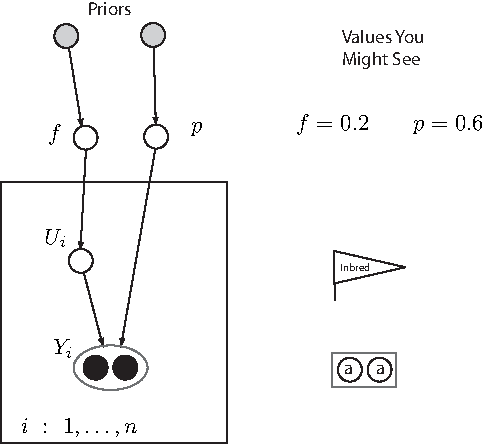
\includegraphics[width=.6\textwidth]{illus/InbreedingDAG.pdf}
\end{center}
\ldots makes it fairly easy to envision how Gibbs updates for \textcolor{Violet}{$p$} and \textcolor{Green}{$\bm{U}$} would proceed.  \hfill\fbox{Computer Demo}







\newslide{DAG notation and terminology}
\begin{center}
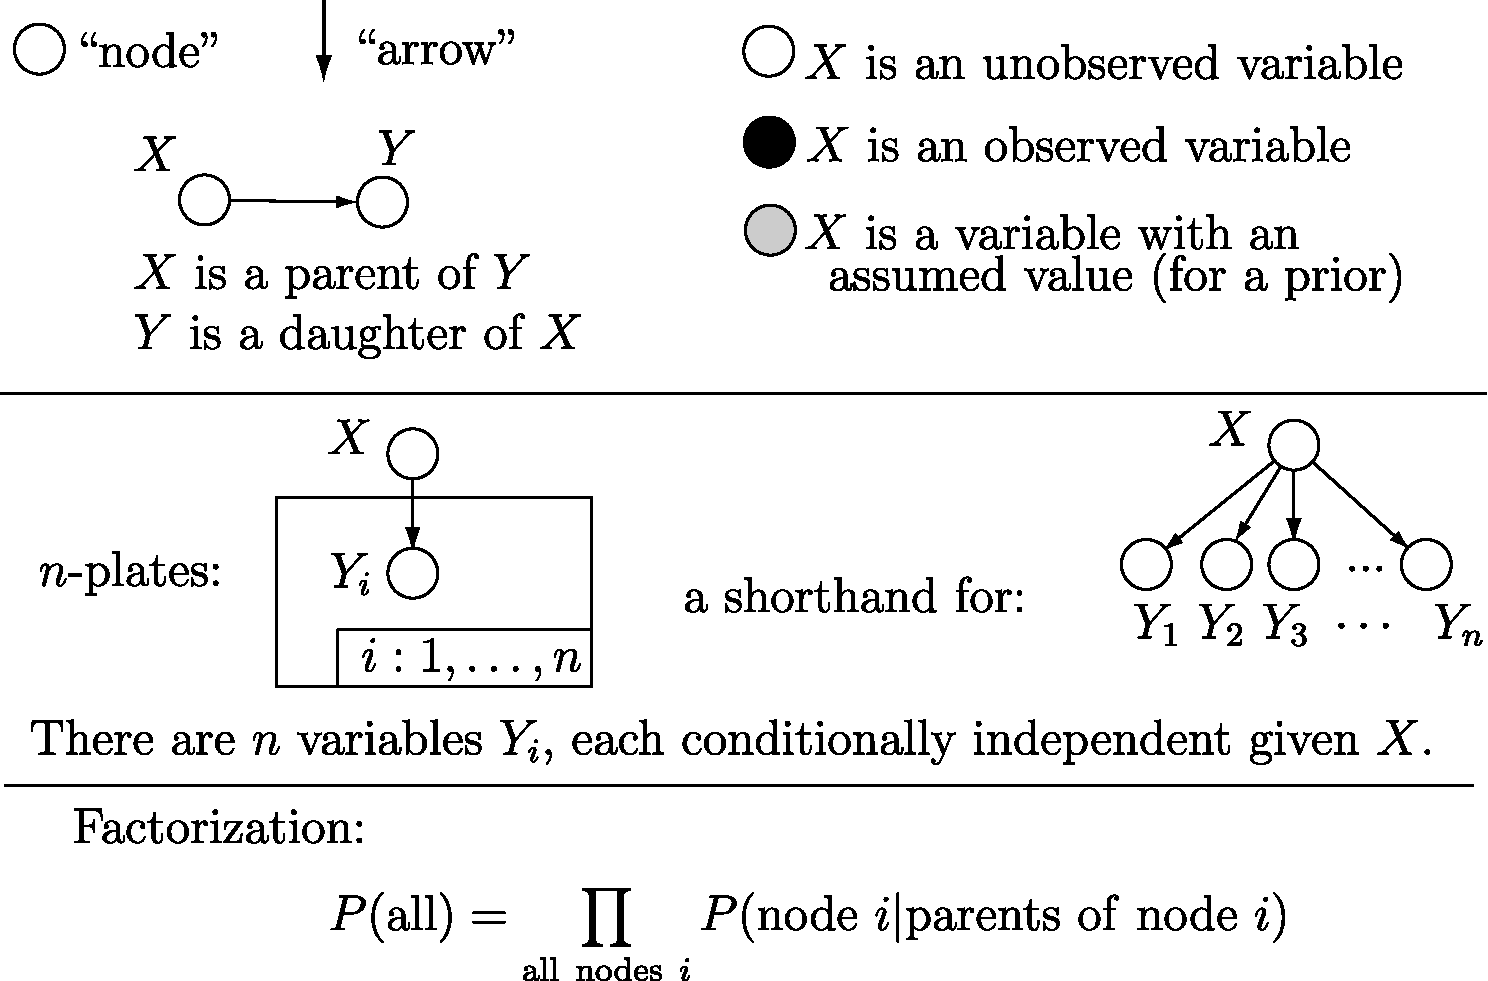
\includegraphics[width=\textwidth]{illus/dagnotat.pdf}
\end{center}





\newslide{A reminder that all inference is conditional upon the underlying model\ldots and a small step toward {\em structure}}
\vspace*{-.25in}
\enlargethispage*{1000pt}
\begin{minipage}{.43\textwidth}
We could have attributed the departure from Hardy-Weinberg proportions to a mixture (in the proportions of $\pi=.5$) of two populations with allele frequencies $p_1$ and $p2$, respectively.
\end{minipage}
\hfill
\begin{minipage}{.5\textwidth}
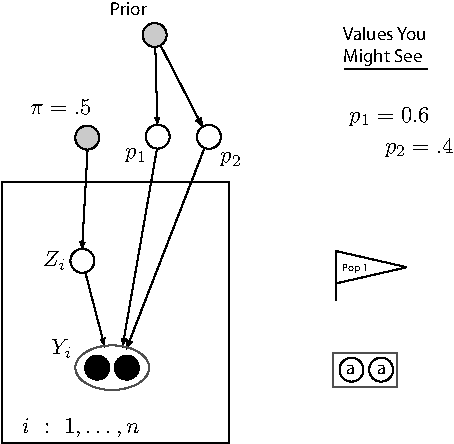
\includegraphics[width=\textwidth]{illus/OneLocusDAG.pdf}
\end{minipage}

This is, in fact, the {\em structure} model with no admixture, $K=2$, and a single locus.

Gibbs sampling is straightforward\ldots\hfill\fbox{Computer Demo}

\newslide{Wrap-Up}
Main Points:
\begin{itemize}
\item In problems where it is useful, MCMC almost always proceeds by proposing changes to a small subset of the variables.
\item There may be many different proposal types.
\begin{itemize}
\item Each proposal type {\em must} satisfy detailed balance.
\item Each proposal type need not make an irreducible chain, BUT
\item All proposals taken together should form an irreducible chain.
\end{itemize}
\item Latent variables may help in factorizing complex joint densities and lend themselves to Gibbs sampling.
\item Simple proposals may be fast to implement, but may not lead to good mixing of the chain.
\item Designing good proposal distributions is where one gets to perform ``art" in implementing MCMC.
\end{itemize}

\end{document}